% Intended LaTeX compiler: pdflatex
\documentclass[10pt,a4paper,UTF8]{article}
\usepackage{zclorg}
\author{zcl.space}
\date{}
\title{LDPC简介}
\hypersetup{
 pdfauthor={zcl.space},
 pdftitle={LDPC简介},
 pdfkeywords={communication  ECC LDPC},
 pdfsubject={本文简单介绍LDPC码},
 pdfcreator={Emacs 25.0.50.1 (Org mode 9.0.5)}, 
 pdflang={English}}
\begin{document}

\maketitle
\tableofcontents
\titlepic{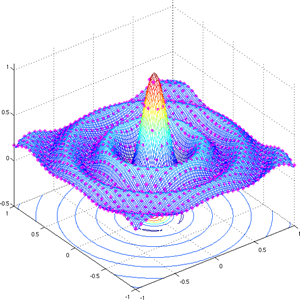
\includegraphics[scale=0.25]{../../img/sinc.PNG}}
1963年,MIT的Gallager发明LDPC(Low-density-Parity-Check)码\footnote{Gallager-Paper}。然而,限于当时计算能力,直到30年后(1996),Mackay 和Neal等人对LDPC码进行了再发现和深入研究,LDPC码才逐渐进入人们视野。目前LDPC码在WIFI,WiMax等各种通信协议中都有广泛的使用。2016年,LDPC被3GPP选为5G数据信道编码方案,标志着LDPC在无线蜂窝网络中占得一席。

本文是关于LDPC码的一系列博文中的第一篇,简单介绍LDPC码的发展历史和基本原理。我将在另外的博文中阐述如何构造LDPC码,译码LDPC码以及LDPC码的其他重要特性。\footnote{Hanzo, Woodard, Robertson   Turbo Decoding and Detection for Wireless Applications     2007 Proceedings of the \{IEEE\} 95, 1178 --1200}





\section{历史}
\label{sec:org9c4bdcc}


LDPC ( Low-density Parity-check,低密度奇偶校验)码是由 Gallager 在1963 年提出的一类具有稀疏校验矩阵的线性分组码 (linear block codes),然而在接下来的 30 年来由于计算能力的不足,它一直被人们忽视。1996年,D MacKay、M Neal 等人对它重新进行了研究,发现 LDPC 码具有逼近香农限的优异性能。并且具有译码复杂度低、可并行译码以及译码错误的可检测性等特点,从而成为了信道编码理论新的研究热点。

Mckay ,Luby 提出的非正则 LDPC 码将 LDPC 码的概念推广。非正则LDPC码 的性能不仅优于正则 LDPC 码,甚至还优于 Turbo 码的性能,是目前己知的最接近香农限的码。

Richardson 和 Urbank 也为 LDPC 码的发展做出了巨大的贡献。首先,他们提出了一种新的编码算法,在很大程度上减轻了随机构造的 LDPC 码在编码上的巨大运算量需求和存储量需求。其次,他们发明了密度演进理论,能够有效的分析出一大类 LDPC 译码算法的译码门限。仿真结果表明,这是一个紧致的译码门限。最后,密度演进理论还可以用于指导非正则 LDPC码 的设计,以获得尽可能优秀的性能。现在Richardson就职于高通,显然是LDPC码进入3GPP eMBB信道的幕后推手之一。Richardson创立的 Flarion公司推出的基于 ASIC 的 Vector-LDPC 解决方案使用了约 260 万门,最高可以支持 50000的码长,0.9 的码率,最大迭代次数为 10,译码器可以达到 10Gbps 的吞吐量,其性能己经非常接近香农限,可以满足目前大多数通信业务的需求。
\section{和Turbo的对比}
\label{sec:org4bad585}


提及LDPC码就不得不提另外一种趋近香农限的码:Turbo码。1993年Berrou等人发明了Turbo码。很快,Turbo的思想在通信系统的各个领域都有深入的应用,最典型的应用便是进入了3G和4G蜂窝网络。关于Turbo的简单介绍,可以参阅我的另外一篇博文。

与Turbo码相比,LDPC码的主要优势有:
\begin{enumerate}
\item LDPC码的译码算法,是一种基于稀疏矩阵的并行迭代译码算法,运算量要低于Turbo码译码算法,并且由于结构并行的特点,在硬件实现上比较容易。因此在大容量通信应用中,LDPC码更具有优势。在深度学习算法横行的今天,运算资源根本不是问题。另外,值得注意的是,基于消息传递算法的LDPC译码算法与机器学习中置信网络算法在本质上毫无二致。目前5G标准要求最高20Gbps的吞吐,对LDPC码来说毫无难度,但是对Turbo码来说却充满挑战。

\item LDPC码的码率可以任意构造,有更大的灵活性。而Turbo码只能通过打孔来达到高码率,这样打孔图案的选择就需要十分慎重的考虑,否则会造成性能上较大的损失。这也是在5G的eMBB选码过程中,Turbo被诟病的一个方面。

\item LDPC码具有更低的错误平层,可以应用于有线通信、深空通信以及磁盘存储工业等对误码率要求更加苛刻的场合。而Turbo码的错误平层远高于 LDPC码,并且目前没有针对Turbo码错误平层的有效应对方法。一种普遍的做法是与其他码级联,形成级联码,但是级联码的实用大大的提高了复杂度。

\item 基于Raptor-like的LDPC码在速率匹配和Harq传输方面有着天然的优势,不需要像Turbo码那样基于一个最低码率(在4G中是1/3,高码率必须通过1/3码率打孔实现。)
\end{enumerate}

与Turbo相比,LDPC的劣势有:

\begin{enumerate}
\item 硬件资源需求比较大。全并行的译码结构对计算单元和存储单元的需求都很大。针对这一问题,已经有多重高效的译码算法提出,他们或者基于行并行,或者基于块并行。

\item 编码比较复杂,更好的编码算法还有待研究。同时,由于需要在码长比较长的情况才能充分体现性能上的优势,所以编码时延也比较大。针对这一问题,提出了 准循环的LDPC码(QC-LDPC码),其编码过程仅仅需要使用寄存器移位即可实现,并且在实现上可以全并行。

\item 相对于Turbo,工业界支持不够。这一问题随着LDPC优良特性越来越被认可,采用LDPC编码的标准越来越多。5G就是一个典型的例子。有人说5G eMBB信道采用LDPC码标志着LDPC码的巅峰和Turbo码的退出。
\end{enumerate}

\section{}
\label{sec:org359425d}
\end{document}
